%%%%%%%%%%%%%%%%%%%%%%%%%%%%%%%%%%%%%%%%%%%%%%%%%%%%%%%%%%%%%%%%%%%%%%%%%%%

\documentclass[a4paper,oneside,12pt]{article}
\usepackage{mystyle}

\begin{document}

\title{\Large\bf Applications of quadratic functions}
\author{%%
  Minh Van Nguyen \\
  \url{mvngu@gmx.com}
}
\date{\today}
\maketitle

\noindent
This document will show you how the quadratic function can be used in
a variety of situations.  The document consists of mostly worked
examples and exercises.  Carefully study the examples to understand
how the quadratic function is used in each case.  Wherever an equation
is given, you should attempt by yourself to derive the equation.  This
not only helps to solidify your understanding of a particular problem,
but also sharpens your problem solving skills.


%%%%%%%%%%%%%%%%%%%%%%%%%%%%%%%%%%%%%%%%%%%%%%%%%%%%%%%%%%%%%%%%%%%%%%%%%%%

\section{Length and width}

This section presents two examples from geometry where the quadratic
function can be used to determine lengths and widths of certain
geometric objects.

\begin{example}
\textbf{Fencing.}
\label{ex:fence_a_rectangular_region}
You want to install a fence around a rectangular region that has an
area of $7$ metres squared.  You want the length of the rectangular
region to be two metres longer than the width.  Calculate the width of
the region.
\end{example}

\begin{solution}
Whenever possible, you should first draw a picture to help you solve a
problem.  In this example, the rectangular region and its dimensions
can be illustrated as shown in
\Figure{fig:rectangular_region_7_metres_squared}.  Since the width of
the region is $w$ metres and its length is $w + 2$ metres, the area of
the region is $(w + 2)w$ metres squared.  However, you also know that
the region has an area of $7$~metres squared, which can be used to
give you the equation
%%
\begin{equation}
\label{eqn:rectangular_region_equation}
(w + 2)w
=
7.
\end{equation}

\begin{figure}[!htbp]
\centering
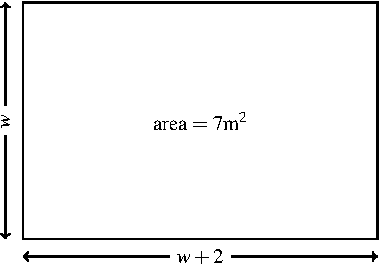
\includegraphics[scale=1]{image/09/rectangular-fence.pdf}
\caption{%%
  A rectangular region whose area is $7$ metres squared.  The width of
  the region is denoted $w$.
}
\label{fig:rectangular_region_7_metres_squared}
\end{figure}

Let's determine all values of $w$ that satisfy
\Equation{eqn:rectangular_region_equation}.  Expand the left-hand side
of \Equation{eqn:rectangular_region_equation} to get $w^2 + 2w = 7$.
Upon moving everything to the left-hand side, you end up with the
quadratic equation
%%
\begin{equation}
\label{eqn:rectangular_region_quadratic}
w^2 + 2w - 7
=
0.
\end{equation}
%%
Writing the left-hand side as $f(w) = w^2 + 2w - 7$,
\Equation{eqn:rectangular_region_quadratic} can also be written as
$f(w) = 0$.  This means that you want to determine all roots of
$f(w)$.  Before calculating the roots of $f(w)$, you investigate
whether $f(w)$ has a unique root, two different roots, or the graph of
$f(w)$ does not intersect the horizontal axis.  This is a job for the
discriminant.  The discriminant of $f(w)$ is $\Delta = 32$.  This is a
positive number so there exists at least one real value of $w$ that
solves \Equation{eqn:rectangular_region_equation}.  Using the
quadratic formula, the roots of $f(w)$ can be written as
$w = -1 \pm 2\sqrt{2}$.  One root of $f(w)$ is given by
\[
w_1
=
2\sqrt{2} - 1
\]
which is positive.  The other root is given by
\[
w_2
=
-2\sqrt{2} - 1
\]
which is negative.  You reject the number $w_2$ because the width of
the rectangular region cannot be a negative number.  To confirm your
decision to reject the root $w_2$, you sketch a graph of $f(w)$ as
shown in \Figure{fig:rectangular_region_quadratic_roots} and note that
$w_2$ is located on the negative half of the $w$-axis, i.e.~the
horizontal axis.  You conclude that the width of the rectangular
region is approximately $2\sqrt{2} - 1 \approx 1.8284$ metres long,
rounded to four decimal places.
\end{solution}

\begin{figure}[!htbp]
\centering
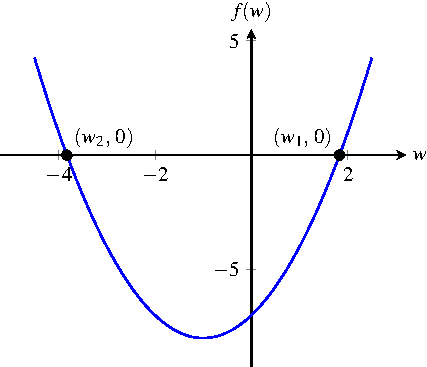
\includegraphics[scale=1]{image/09/a1-b2-cminus7.pdf}
\caption{%%
  Graph of the function $f(w) = w^2 + 2w - 7$.  The two dots indicate
  the two different roots of $f(w)$.
}
\label{fig:rectangular_region_quadratic_roots}
\end{figure}

\begin{exercise}
\label{ex:rectangular_region_discriminant}
In the solution of \Example{ex:fence_a_rectangular_region}, verify
that the discriminant is $\Delta = 32$.
\end{exercise}
%%
\ifbool{showSolution}{
\begin{solution}
In the equation $f(w) = w^2 + 2w - 7$, you have the values $a = 1$,
$b = 2$, and $c = -7$.  Use \Definition{def:discriminant} to see that
the discriminant of $f(w)$ is
%%
\begin{align*}
\Delta
&=
2^2 - 4(1)(-7) \\[4pt]
&=
4 + 28 \\[4pt]
&=
32
\end{align*}
%%
as required.
\end{solution}
}{}

\begin{exercise}
In the solution of \Example{ex:fence_a_rectangular_region}, verify
that the roots of $f(w)$ can be written as $w = -1 \pm 2\sqrt{2}$.
\end{exercise}
%%
\ifbool{showSolution}{
\begin{solution}
You have the equation $f(w) = w^2 + 2w - 7$, whose roots can be
calculated by using the quadratic formula.  The discriminant of $f(w)$
is known to be $\Delta = 32$, as verified in
\Exercise{ex:rectangular_region_discriminant}, so the roots are
%%
\begin{align*}
w
&=
\frac{
  -2 \pm \sqrt{\Delta}
}{
  2(1)
} \\[4pt]
&=
\frac{
  -2 \pm \sqrt{2 \times 4^2}
}{
  2
} \\[4pt]
&=
\frac{
  -2 \pm 4\sqrt{2}
}{
  2
} \\[4pt]
&=
\frac{
  2(-1 \pm 2\sqrt{2})
}{
  2
} \\[4pt]
&=
-1 \pm 2\sqrt{2}
\end{align*}
%%
as required.
\end{solution}
}{}

\begin{example}
\label{ex:running_ants}
\textbf{Ant race.}
Two ants are next to each other.  Ant $A$ runs eastward at a rate of
two centimetres per second.  After one second since ant $A$ started
running, ant $B$ runs northward also at the same rate.  How long since
ant $A$ started running does it take for both ants to be five
centimetres apart?
\end{example}

\begin{solution}
As in \Example{ex:fence_a_rectangular_region}, you should first draw a
picture that can help you in solving the problem.  Denote by $t$ the
time in seconds and use $t$ to represent the amount of time that ant
$A$ runs.  Since ant $A$ runs in the eastern direction at two
centimetres per second, after $t$ seconds the ant would have covered a
horizontal distance of $2t$ centimetres.  When ant $A$ starts running,
ant $B$ is still at the starting position and must wait one second
before it starts to run in the northern direction.  The amount of time
that ant $B$ runs is one second less than the amount of time that ant
$A$ runs.  In other words, the duration of time that ant $B$ runs can
be written as $t - 1$ seconds, after which the ant would have
travelled a vertical distance of $2(t - 1)$ centimetres.  The
situation is illustrated in \Figure{fig:running_ants_triangle}.

\begin{figure}[!htbp]
\centering
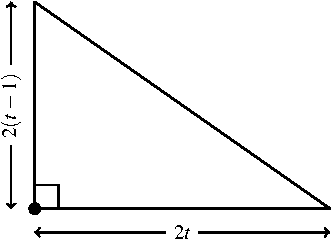
\includegraphics[scale=1]{image/09/running-ants.pdf}
\caption{%%
  A right-angled triangle that represents the directions in which two
  ants run.  The dot indicates the starting position of the ants.  The
  variable $t$ denotes time in seconds.  After $t$ seconds, the
  distance between the ants is represented by the length of the
  hypotenuse.
}
\label{fig:running_ants_triangle}
\end{figure}

Let's now formulate the problem as an equation.  The horizontal and
vertical distances travelled by both ants can be represented as the
base and height, respectively, of the right-angled triangle in
\Figure{fig:running_ants_triangle}.  After $t$ seconds have passed,
the distance between the ants is represented by the length of the
hypotenuse of the triangle.  Using Pythagoras' theorem, the problem
can be formulated as the quadratic equation
%%
\begin{equation}
\label{eqn:running_ants_quadratic_equation}
8t^2 - 8t + 4
=
25.
\end{equation}

The problem now is to determine all values of $t$ that satisfy
\Equation{eqn:running_ants_quadratic_equation}.  Note that the
equation can also be written as
\[
8t^2 - 8t - 21
=
0.
\]
Writing $f(t) = 8t^2 - 8t - 21$,
\Equation{eqn:running_ants_quadratic_equation} is equivalent to the
equation $f(t) = 0$, hence the values of $t$ that satisfy
\Equation{eqn:running_ants_quadratic_equation} are the same as the
roots of $f(t)$.  The quadratic formula shows that the roots of $f(t)$
are
%%
\begin{equation}
\label{eqn:running_ants_roots}
t_1
=
\frac{1}{2}
+
\frac{\sqrt{46}}{4}
%%
\qquad
\text{and}
\qquad
%%
t_2
=
\frac{1}{2}
-
\frac{\sqrt{46}}{4}.
\end{equation}
%%
You reject the root $t_2$ because it is negative.  A negative value of
time does not make sense in the context of the problem.  Therefore the
ants would be five centimetres apart after approximately
$\frac{1}{2}
+
\frac{\sqrt{46}}{4}
\approx
2.1956$
seconds~(rounded to four decimal places) since ant $A$ started running.
\end{solution}

\begin{exercise}
Explain why \Example{ex:running_ants} can be represented as
\Equation{eqn:running_ants_quadratic_equation}.
\end{exercise}
%%
\ifbool{showSolution}{
\begin{solution}
From \Figure{fig:running_ants_triangle} you know that after $t$
seconds, ant $A$ would have travelled $2t$ centimetres and ant $B$
would have travelled $2(t - 1)$ centimetres.  These numbers are the
base and height, respectively, of a right-angled triangle.  After $t$
seconds, the distance between the ants is represented by the  length
of the hypotenuse in \Figure{fig:running_ants_triangle}.  You want to
know when the ants are $5$ centimetres apart, so the hypotenuse is $5$
centimetres.  By Pythagoras' theorem, the three sides of the
right-angled triangle are related by the equation
\[
(2t)^2 + \bigparen{2 (t - 1)}^2
=
5^2.
\]
Upon expanding the parentheses, the equation can be written as
\[
4t^2 + (2t - 2)^2
=
25.
\]
Expand the remaining pair of parentheses to get
\[
4t^2 + 4t^2 - 8t + 4
=
25.
\]
After collecting like terms, you end up with
\Equation{eqn:running_ants_quadratic_equation}.
\end{solution}
}{}

\begin{exercise}
In the solution to \Example{ex:running_ants}, verify that the roots of
$f(t)$ are those given by~\eqref{eqn:running_ants_roots}.
\end{exercise}
%%
\ifbool{showSolution}{
\begin{solution}
You have the quadratic function $f(t) = 8t^2 - 8t - 21$.  Using the
quadratic formula, the roots of $f(t)$ are
%%
\begin{align*}
t
&=
\frac{
  -(-8) \pm \sqrt{(-8)^2 - 4(8)(-21)}
}{
  2(8)
} \\[4pt]
&=
\frac{
  8 \pm \sqrt{736}
}{
  16
} \\[4pt]
&=
\frac{
  8 \pm \sqrt{4^2 \times 2 \times 23}
}{
  16
} \\[4pt]
&=
\frac{
  8 \pm 4\sqrt{46}
}{
  16
} \\[4pt]
&=
\frac{
  4 \parenthesis*{2 \pm \sqrt{46}}
}{
  4^2
} \\[4pt]
&=
\frac{
  2 \pm \sqrt{46}
}{
  4
} \\[4pt]
&=
\frac{1}{2}
\pm
\frac{\sqrt{46}}{4}
\end{align*}
%%
which are the same as those given by~\eqref{eqn:running_ants_roots}.
\end{solution}
}{}


%%%%%%%%%%%%%%%%%%%%%%%%%%%%%%%%%%%%%%%%%%%%%%%%%%%%%%%%%%%%%%%%%%%%%%%%%%%

\section{Largest or smallest}

This section considers two optimisation problems.  Such problems
require you to maximise or minimise a particular function.  In the
context of a quadratic function, the optimised value of the function
is the function's vertex.

\begin{example}
\label{eg:largest_area_rectangle}
\textbf{Largest area.}
A rectangle has a perimeter of ten metres.
%%
\begin{packedenum}
\item\label{subex:largest_area_perimeter_area}
  Derive a function for the area of the rectangle.

\item\label{subex:largest_area_of_rectangle}
  Calculate the largest area that the rectangle can have.
\end{packedenum}
\end{example}

\begin{solution}
\solutionpart{subex:largest_area_perimeter_area}
As in \Examples{ex:fence_a_rectangular_region}{ex:running_ants}, you
should draw a picture to help you solve the problem.  Let $\ell$ and
$w$ be the length and width, respectively, of the rectangle.  Since
the rectangle has a perimeter of ten metres, the equation for the
perimeter can be written as
\[
2\ell + 2w
=
10
\]
and thus the length can be written as $\ell = 5 - w$.  The length and
width of the rectangle are illustrated in
\Figure{fig:largest_area_rectangle}.  Using the information from
\Figure{fig:largest_area_rectangle}, the area of the rectangle can be
written as the function
\[
f(w)
=
(5 - w)w
\]
which after expansion becomes $f(w) = -w^2 + 5w$.

\begin{figure}[!htbp]
\centering
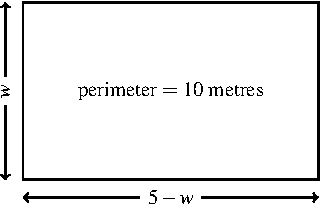
\includegraphics[scale=1]{image/09/largest-area.pdf}
\caption{%%
  A rectangle whose perimeter is ten metres.  The width is denoted as
  $w$ and the length is $5 - w$.
}
\label{fig:largest_area_rectangle}
\end{figure}

\begin{figure}[!htbp]
\centering
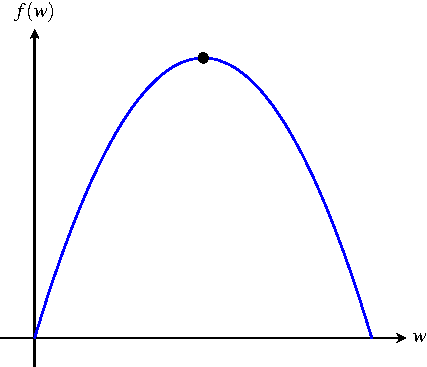
\includegraphics[scale=1]{image/09/rectangle-area.pdf}
\caption{%%
  The area $f(w) = (5 - w) w$ of a rectangle as a function of its
  width $w$.  The vertex of the parabola is the highest point in the
  graph of $f(w)$.  Here, the vertex is also the point at which the
  value of $f(w)$, or the area, is largest.
}
\label{fig:largest_area_graph_parabola}
\end{figure}

\solutionpart{subex:largest_area_of_rectangle}
\Figure{fig:largest_area_graph_parabola} shows a graph of the function
$f(w)$.  Note the highest point in the graph.  The horizontal
coordinate~(i.e.~the value of $w$) gives you the width of the
rectangle.  The vertical coordinate~(i.e.~the value of $f(w)$) gives
you the corresponding area of the rectangle.  So the largest area of
the rectangle occurs at the vertex in the graph of $f(w)$.  The
horizontal coordinate of the vertex is
\[
w
=
\frac{5}{2}.
\]
In other words, the largest value of the function $f(w)$ occurs when
the width is $w = 5 / 2 = 2.5$ metres.  What about the actual value of
$f(w)$?  Substitute $w = 5 / 2$ into $f(w)$ to get
\[
f(5/2)
=
\frac{25}{4}.
\]
This tells you that the largest area the rectangle can have is
$25 / 4 = 6.25$ metres squared.
\end{solution}

\begin{exercise}
In \Example{eg:largest_area_rectangle}, explain why the length of the
rectangle can be written as $\ell = 5 - w$.
\end{exercise}

\ifbool{showSolution}{
\begin{solution}
Note that the perimeter of the rectangle can be written as
\[
2\ell + 2w
=
10
\]
where $\ell$ and $w$ are the length and width, respectively, of the
rectangle.  You can also write the last equation as
$2(\ell + w) = 10$, which can be simplified to $\ell + w = 5$.  The
length of the rectangle can now be written as $\ell = 5 - w$.
\end{solution}
}{}

\begin{exercise}
In \Example{eg:largest_area_rectangle}, verify that the vertex of the
function $f(w)$ occurs at the point
$\tuple{\frac{5}{2}}{\frac{25}{4}}$.
\end{exercise}

\ifbool{showSolution}{
\begin{solution}
The horizontal coordinate of the vertex is
%%
\begin{align*}
w
&=
-\frac{5}{2(-1)} \\[4pt]
&=
\frac{-5}{-2} \\[4pt]
&=
\frac{5}{2}.
\end{align*}
%%
To get the vertical coordinate of the vertex, substitute $w = 5 / 2$
into $f(w)$ to get
%%
\begin{align*}
f(5/2)
&=
\parenthesis*{5 - \frac{5}{2}} \frac{5}{2} \\[4pt]
&=
\parenthesis*{\frac{10}{2} - \frac{5}{2}} \frac{5}{2} \\[4pt]
&=
\frac{5}{2} \times \frac{5}{2} \\[4pt]
&=
\frac{25}{4}
\end{align*}
%%
as required.
\end{solution}
}{}

\begin{example}
\label{eg:smallest_product}
\textbf{Smallest product.}
Let $x$ and $y$ be two numbers such that when you subtract $y$ from
$x$ you get $1$.  Determine the smallest value of the product $xy$.
\end{example}

\begin{solution}
From the statement of the problem, you have the equation
\[
x - y
=
1
\]
and so $y$ can be written as $y = x - 1$.  The product of $x$ and $y$
can be written as the quadratic function $f(x) = x^2 - x$, a graph of
which is shown in \Figure{fig:graph_smallest_product}.

\begin{figure}[!htbp]
\centering
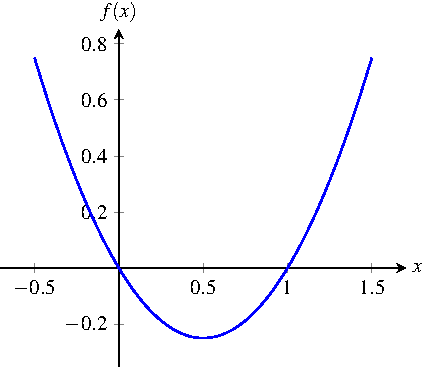
\includegraphics[scale=1.2]{image/09/smallest-product.pdf}
\caption{%%
  A graph of the function $f(x) = x^2 - x$, whose vertex is its lowest
  point.
}
\label{fig:graph_smallest_product}
\end{figure}

As $f(x)$ is a function that represents the product of $x$ and $y$,
the graph in \Figure{fig:graph_smallest_product} shows that the
smallest value of the product $xy$ occurs at the vertex of $f(x)$.
The horizontal coordinate of the vertex is
\[
x
=
\frac{1}{2}.
\]
Hence the vertical coordinate of the vertex is
\[
f(1/2)
=
-\frac{1}{4}.
\]
This tells you that the smallest value of the product $xy$ is
$-\frac{1}{4}$ and this least value occurs when $x = 1/2$.
\end{solution}

\begin{exercise}
In \Example{eg:smallest_product}, explain why $y$ can be written as
$y = x - 1$.
\end{exercise}

\ifbool{showSolution}{
\begin{solution}
You have the equation $x - y = 1$.  Move everything to the left-hand
side and you get $x - y - 1 = 0$.  Upon moving $y$ to the right-hand
side you end up with $x - 1 = y$.
\end{solution}
}{}

\begin{exercise}
In \Example{eg:smallest_product}, show that the product $xy$ can be
written as the function $f(x) = x^2 - x$.
\end{exercise}

\ifbool{showSolution}{
\begin{solution}
Since $y = x - 1$, the product $xy$ can be written as
\[
xy
=
x(x - 1).
\]
Use the distributive laws to expand the right-hand side and you get
$x^2 - x$.
\end{solution}
}{}

\begin{exercise}
In \Example{eg:smallest_product}, verify that the vertex of the
function $f(x) = x^2 - x$ is the point
$\tuple{\frac{1}{2}}{-\frac{1}{4}}$.
\end{exercise}

\ifbool{showSolution}{
\begin{solution}
The horizontal coordinate of the vertex of $f(x)$ is
%%
\begin{align*}
x
&=
-\frac{-1}{2(1)} \\[4pt]
&=
\frac{1}{2}.
\end{align*}
%%
The vertical coordinate of the vertex is
%%
\begin{align*}
f(1/2)
&=
\parenthesis*{\frac{1}{2}}^2 - \frac{1}{2} \\[4pt]
&=
\frac{1}{4} - \frac{2}{4} \\[4pt]
&=
\frac{1 - 2}{4} \\[4pt]
&=
-\frac{1}{4}
\end{align*}
%%
as required.
\end{solution}
}{}


%%%%%%%%%%%%%%%%%%%%%%%%%%%%%%%%%%%%%%%%%%%%%%%%%%%%%%%%%%%%%%%%%%%%%%%%%%%

\section{Free fall}

This section considers an example from physics.  You throw a small
ball straight up into the air.  The ball travels upward in a straight
line for some time, reaches a maximum height, and then falls to the
ground.  Other than throwing the ball upward, you do not interfere
with the movement of the ball, but allow the forces of gravity and air
drag~(air resistance) to act on the ball.  In many cases, the force of
air drag can be ignored.  For now you only need to take into account
the force of gravity.  When the ball is allowed to move vertically as
described above, the motion of the ball is an example of
\emph{free fall}.

The position of the ball changes with time.  But precisely in what
way?  To analyse the position of the ball, let's make various
assumptions.  Denote by $t$ the time in seconds and let $f(t)$ be the
height in metres of the ball.  The \emph{initial height} of the ball
is the ball's height above ground level before the ball moves upward.
When you hold the ball in your hand just before you throw it upward,
the initial height of the ball is the distance~(in metres) from your
hand to the ground.  If the ball is on the ground before it moves
upward, its initial height is zero metres.  Let $h$ be the initial
height of the ball.  The \emph{initial velocity} of the ball is the
speed in metres per second with which the ball is thrown upward.
Denote the initial velocity of the ball by $v$.  The force of gravity
acts on the ball in a downward manner.  This is because gravity tends
to pull an object downward towards the centre of the Earth.  The force
of gravity is usually written as $g$ and its value is the constant of
$9.8$ metres per second squared.  To analyse the position of the ball,
you must take into account the initial height of the ball, the upward
distance it travels as time passes, and the downward force of gravity.
The position of the ball above ground level can be approximated by the
quadratic function
%%
\begin{equation}
\label{eqn:position_of_object_under_free_fall}
f(t)
=
-\frac{1}{2} gt^2 + vt + h.
\end{equation}

\begin{example}
\label{ex:spring_ball}
\textbf{Boing boing.}
A spring is located at ground level and can shoot a ball upward at an
initial velocity of $10$ metres per second.
%%
\begin{packedenum}
\item\label{ex:spring_ball_graph}
  Write a function for the position of the ball and graph the
  function.

\item\label{ex:spring_ball_time_to_maximum_height}
  Determine the amount of time~(in seconds) required for the ball to
  reach maximum height.  Calculate the maximum height~(in metres) that
  the ball reaches.

\item\label{ex:spring_ball_time_hit_ground}
  When will the ball reach the ground?
\end{packedenum}
\end{example}

\begin{solution}
\solutionpart{ex:spring_ball_graph}
You know that the force of gravity is $g = 9.8$ metres per second
squared.  The initial velocity is $v = 10$ metres per second.  Since
the spring is located at ground level, let's assume that the initial
height of the ball is $h = 0$ metres.  Substitute these values into
\Equation{eqn:position_of_object_under_free_fall} and simplify the
result to get
\[
f(t)
=
-\frac{49}{10}t^2 + 10t
\]
whose graph is shown in \Figure{fig:spring_ball_graph}.  This is a
rough sketch that illustrates three points on which you should
concentrate.  First is the point at the origin $\tuple{0}{0}$ that
tells you the initial height of the ball at time $t = 0$ before the
ball is shot upward.  Next is the vertex of the function $f(t)$, which
in this example is the highest point $\tuple{a}{f(a)}$ of the graph of
$f(t)$.  The vertex $\tuple{a}{f(a)}$ tells you that the ball reaches
its maximum height of $f(a)$ metres above the ground at time $t = a$
seconds after being shot upward by the spring.  The third point
$\tuple{b}{0}$ tells you approximately how long the ball is in the air
before it lands on the ground.  You do not yet know the values of $a$
and $b$.  This is just a rough sketch to help you understand the
example.

\begin{figure}[!htbp]
\centering
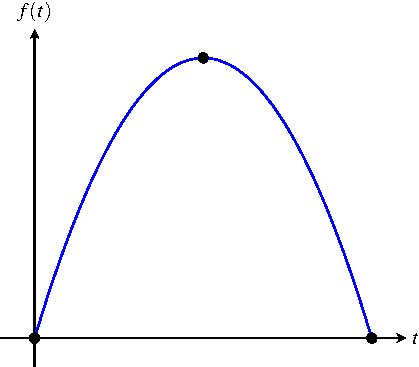
\includegraphics[scale=1]{image/09/spring-ball.pdf}
\caption{%%
  The height of a ball as a function of time.  Here, time $t$ is
  measured in seconds and the height $f(t)$ of the ball is measured in
  metres above the ground.
}
\label{fig:spring_ball_graph}
\end{figure}

\solutionpart{ex:spring_ball_time_to_maximum_height}
You know that the vertex~(i.e. highest point) of the graph of $f(t)$
occurs at $t = 50/49$.  This means that the ball reaches its maximum
height above the ground at approximately $t = 50/49 \approx 1.0204$
seconds~(rounded to four decimal places) after being shot up by the
spring.  The maximum height that the ball reaches is
$f(50 / 49) = 250 / 49$, which is approximately $5.1020$ metres above
the ground, rounded to four decimal places.

\solutionpart{ex:spring_ball_time_hit_ground}
You can use the quadratic formula to calculate the time at which the
ball hits the ground.  However, the following is a simple method that
does not use the quadratic formula.  Note that the function $f(t)$ can
be factorised as
%%
\begin{align*}
f(t)
&=
-\frac{49}{10} t^2 + 10t \\[4pt]
&=
\parenthesis*{-\frac{49}{10} t + 10} t \\[4pt]
&=
\parenthesis*{10 - \frac{49}{10} t} t.
\end{align*}
%%
Since the roots of $f(t)$ are those values of $t$ such that the
equation $f(t) = 0$ is true, this is the same as determining the
values of $t$ such that the following equation is true:
%%
\begin{equation}
\label{eqn:spring_ball_equation_factored}
\parenthesis*{10 - \frac{49}{10} t} t
=
0.
\end{equation}
%%
Equation~\eqref{eqn:spring_ball_equation_factored} is true when
$t = 0$.  However, when $t = 0$ the ball is at its initial height of
zero metres above ground level and so the point $\tuple{0}{0}$ is the
starting position of the ball when it is initially on the ground.  In
other words, you can ignore the root $t = 0$ of $f(t)$.  Let's
consider the other factor $10 - \frac{49}{10} t$.  If you have
$10 - \frac{49}{10} t = 0$, then
\Equation{eqn:spring_ball_equation_factored} will also be true.  Now
you must solve the equation $10 - \frac{49}{10} t = 0$ for $t$.  Doing
so gives you the root $t = 100 / 49$.  Therefore the ball will reach
the ground at approximately $t = 100 / 49 \approx 2.0408$ seconds
after being shot up by the spring.
\end{solution}

\begin{exercise}
You will verify the solution of \Example{ex:spring_ball}.
%%
\begin{packedenum}
\item\label{subex:spring_ball_height_function}
  Show that the height of the ball can be written as
  $f(t) = -\frac{49}{10} t^2 + 10t$.

\item\label{subex:spring_ball_highest_point}
  Show that the ball reaches its maximum height at $t = 50 / 49$
  seconds after being shot up.  Also show that the maximum height of
  the ball is $f(50 / 49) = 250 / 49$ metres above the ground.

\item\label{subex:spring_ball_quadratic_formula}
  Use the quadratic formula to calculate the roots of $f(t)$.
\end{packedenum}
\end{exercise}
%%
\ifbool{showSolution}{
\begin{solution}
\solutionpart{subex:spring_ball_height_function}
You know that the force of gravity is $g = 9.8 = 49/5$ metres per
second squared, the initial velocity of the ball is $v = 10$ metres
per second, and the initial height of the ball is $h = 0$ metres above
ground level.  Substitute these values into
\Equation{eqn:position_of_object_under_free_fall} to obtain
%%
\begin{align*}
f(t)
&=
-\frac{49}{5} \times \frac{1}{2} t^2 + 10t + 0 \\[4pt]
&=
-\frac{49}{10} t^2 + 10t.
\end{align*}

\solutionpart{subex:spring_ball_highest_point}
The horizontal coordinate of the vertex of $f(t)$ is
%%
\begin{align*}
t
&=
-\frac{10}{2 \times \parenthesis*{-\frac{49}{10}}} \\[4pt]
&=
\frac{10}{\frac{49}{5}} \\[4pt]
&=
10 \times \frac{5}{49} \\[4pt]
&=
\frac{50}{49}.
\end{align*}
%%
Then the vertical coordinate of the vertex is
%%
\begin{align*}
f(50 / 49)
&=
-\frac{49}{10} \parenthesis*{\frac{50}{49}}^2
+
10\parenthesis*{\frac{50}{49}} \\[4pt]
&=
-\frac{49}{10} \times \frac{50^2}{49^2}
+
\frac{10 \times 50}{49} \\[4pt]
&=
-\frac{5 \times 50}{49}
+
\frac{10 \times 50}{49} \\[4pt]
&=
\frac{
  50(10 - 5)
}{
  49
} \\[4pt]
&=
\frac{
  250
}{
  49
}.
\end{align*}
%%

\solutionpart{subex:spring_ball_quadratic_formula}
Using the quadratic formula results in
%%
\begin{align*}
t
&=
\frac{
  -(10) \pm \sqrt{10^2 - 4\parenthesis*{-\frac{49}{10}} (0)}
}{
  2 \parenthesis*{-\frac{49}{10}}
} \\[4pt]
&=
\frac{
  -10 \pm \sqrt{10^2}
}{
  -\frac{49}{5}
} \\[4pt]
&=
\frac{
  -10 \pm 10
}{
  -\frac{49}{5}
}.
\end{align*}
%%
The roots of $f(t)$ are
\[
t_1
=
\frac{
  -10 + 10
}{
  -\frac{49}{5}
}
=
0
%%
\qquad
\text{and}
\qquad
%%
t_2
=
\frac{
  -10 - 10
}{
  -\frac{49}{5}
}
=
\frac{100}{49}.
\]

\end{solution}
}{}


\newpage
%%%%%%%%%%%%%%%%%%%%%%%%%%%%%%%%%%%%%%%%%%%%%%%%%%%%%%%%%%%%%%%%%%%%%%%%%%%

\section*{Problem}

\begin{problem}
\item If you have not done so, read the following articles:

  \begin{packeditem}
  \item \emph{101 uses of a quadratic equation}

  \item \emph{101 uses of a quadratic equation: Part II}
  \end{packeditem}

  Try to understand as much as you can the uses of the quadratic
  function.

\item In your backyard, you want to create a rectangular plot of land
  for some plants.  You want the area of the plot to be $8$ metres
  squared.  You have not yet decided on the length of the plot of
  land.  However, you know that if the plot has a length of $\ell$
  metres, then you want the width to be $\ell - 3$ metres.  Calculate
  the length of the rectangular plot of land for your plants such that
  the area of the plot is $8$ metres squared.
\ifbool{showSolution}{
\begin{solution}
You should first draw a picture to help you solve the problem.  The
picture should be a rectangle whose length and width are $\ell$ and
$\ell - 3$, respectively.  The area of the rectangle is then
$(\ell - 3)\ell$.  Since you know that the plot of land has an area of
$8$ metres squared, it follows that you have the equation
%%
\begin{equation}
\label{eqn:area_rectangular_garden}
(\ell - 3)\ell
=
8.
\end{equation}
%%
Use the distributive laws to expand the left-hand side to get
$\ell^2 - 3\ell = 8$.  In the latter equation, move everything to the
left-hand side to get
\[
\ell^2 - 3\ell - 8
=
0.
\]
If you define the function $f(\ell) = \ell^2 - 3\ell - 8$, then the
equation $f(\ell) = 0$ says that you want to determine all values of
$\ell$ such that \Expression{eqn:area_rectangular_garden} is true.  In
other words, you want to calculate all the roots of the quadratic
function $f(\ell)$.  Use the quadratic formula to see that the roots
of $f(\ell)$ are
\[
\ell_1
=
\frac{
  3 + \sqrt{41}
}{
  2
}
%%
\qquad
\text{and}
\qquad
%%
\ell_2
=
\frac{
  3 - \sqrt{41}
}{
  2
}
\]
of which only $\ell_1$ is positive.  Conclude that the required length
of the rectangular plot of land is approximately
$\frac{
  3 + \sqrt{41}
}{
  2
}
\approx
4.7016$
metres, rounded to four decimal places.
\end{solution}
}{}

\item A right-angled triangle has a base and height of lengths $b$ and
  $b + 1$ metres, respectively.  Suppose the hypotenuse has a length
  of $b + 2$ metres.
  %%
  \begin{packedenum}
  \item\label{subprob:right_triangle_root_exists}
    Without actually calculating a specific value of $b$, show that
    there is a real value of $b$ that satisfies the above conditions.

  \item\label{subprob:right_triangle_base}
    Determine a positive value of $b$ such that the above conditions
    are satisfied.

  \item\label{subprob:right_triangle_three_sides}
    Determine the length of each side of the triangle.
  \end{packedenum}
\ifbool{showSolution}{
\begin{solution}
\solutionpart{subprob:right_triangle_root_exists}
You should draw a picture to help you solve the problem.  The picture
should be a right-triangle whose base has length $b$ metres, whose
height is $b + 1$ metres, and the hypotenuse has a length of $b + 2$
metres.  To calculate a value of $b$ that satisfies the above
conditions, you can use Pythagoras' theorem to obtain the equation
\[
b^2 + (b + 1)^2
=
(b + 2)^2.
\]
Use the distributive laws to expand both sides of the equation and you
end up with the equivalent equation
\[
2b^2 + 2b + 1
=
b^2 + 4b + 4.
\]
In the last equation, move everything to the left-hand side and you
get
%%
\begin{equation}
\label{eqn:right_triangle_roots}
b^2 - 2b - 3
=
0.
\end{equation}
%%
If you define the function $f(b) = b^2 - 2b - 3$, then
\Equation{eqn:right_triangle_roots} can be written as
$f(b) = 0$, which says that you want to determine all roots of
$f(b)$.  Since $f(b)$ is a quadratic function, you can use its
discriminant to see whether there is a real value of $b$ such that
\Expression{eqn:right_triangle_roots} is true.  The discriminant of
$f(b)$ is
\[
\Delta
=
(-2)^2 - 4(1)(-3)
=
16
\]
which is positive.  Therefore there exists a real value of $b$ such
that \Expression{eqn:right_triangle_roots} is true.

\solutionpart{subprob:right_triangle_base}
Use the quadratic formula to see that the roots of $f(b)$ are given by
\[
b_1
=
3
%%
\qquad
\text{and}
\qquad
%%
b_2
=
-1
\]
of which only $b_1$ is positive.  Thus $b = 3$ is a positive number
that meets the requirements of the problem statement.

\solutionpart{subprob:right_triangle_three_sides}
From \Part{subprob:right_triangle_base} you have $b = 3$.  Then the
height of the triangle has a length of $b + 1 = 4$ metres and the
hypotenuse has a length of $b + 2 = 5$ metres.
\end{solution}
}{}

\item A triangle has a base of $b$ metres and a height of $b + 2$
  metres.  Determine a positive value of $b$ such that the triangle
  has an area of $3$ metres squared.
\ifbool{showSolution}{
\begin{solution}
If you know the base $b$ and height $h$ of a triangle, then the
triangle has an area of $\frac{bh}{2}$.  For the triangle in the
problem statement, the area of the triangle can be written as the
equation
%%
\begin{equation}
\label{eqn:area_of_general_triangle}
\frac{b(b+2)}{2}
=
3
\end{equation}
%%
which can also be written as
\[
b(b + 2)
=
6.
\]
In the latter equation, use the distributive laws to expand the
left-hand side to get
\[
b^2 + 2b
=
6.
\]
Upon moving everything to the left-hand side, you end up with
\[
b^2 + 2b - 6
=
0
\]
which is the same as \Equation{eqn:area_of_general_triangle}.  By
defining the function
\[
f(b)
=
b^2 + 2b - 6
\]
\Equation{eqn:area_of_general_triangle} can be written as
$f(b) = 0$, which asks you to determine all roots of $f(b)$.  Since
$f(b)$ is a quadratic function, use the quadratic formula to see that
the roots of $f(b)$ are
\[
b_1
=
\sqrt{7} - 1
%%
\qquad
\text{and}
\qquad
%%
b_2
=
-\sqrt{7} - 1
\]
of which only $b_1$ is positive.  Therefore if the base of the
triangle is $b = \sqrt{7} - 1$ metres and the height is
$b + 2 = \sqrt{7} + 1$ metres, then the triangle will have an area of
$3$ metres squared.
\end{solution}
}{}

\item Let $x$ and $y$ be two numbers such that their sum is $2$.
  Determine the maximum value of the product $xy$.
\ifbool{showSolution}{
\begin{solution}
You have the equation $x + y = 2$, which after solving for $y$ results
in $y = 2 - x$.  The product $xy$ can be written as
\[
xy
=
x(2 - x).
\]
Use the distributive laws to expand the right-hand side and you obtain
the function $f(x) = -x^2 + 2x$, a graph of which is shown in
\Figure{fig:largest_product_xy}.

\begin{figure}[!htbp]
\centering
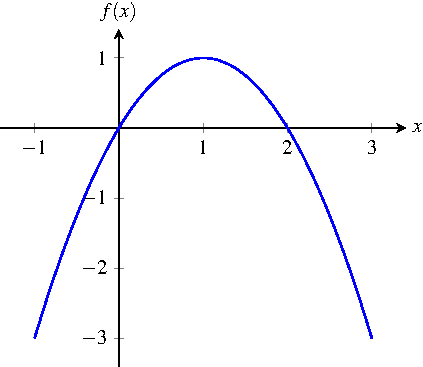
\includegraphics[scale=1.2]{image/09/largest-product.pdf}
\caption{%%
  A graph of the function $f(x) = -x^2 + 2x$.  The vertex of the
  function is the highest point in its graph.
}
\label{fig:largest_product_xy}
\end{figure}

From \Figure{fig:largest_product_xy}, you see that the largest value
of the product $xy = f(x)$ occurs at the vertex of $f(x)$.  The
horizontal coordinate of the vertex is
\[
x
=
-\frac{2}{2(-1)}
=
\frac{-2}{-2}
=
1.
\]
The vertical coordinate of the vertex is
\[
f(1)
=
-(1)^2 + 2(1)
=
-1 + 2
=
1.
\]
In other words, the largest value of the product $xy$ is $1$ and this
maximum value occurs when $x = 1$.
\end{solution}
}{}

\item A rectangle has a perimeter of $p > 0$.  Its length and width
  are $\ell$ and $w$, respectively.
  %%
  \begin{packedenum}
  \item\label{subprob:rectangle_length_w_p}
    Express the length in terms of the perimeter and width of the
    rectangle.

  \item\label{subprob:rectangle_maximum_area}
    Determine the maximum area of the rectangle.

  \item\label{subprob:rectangle_maximum_area_is_square}
    Show that the maximum area is obtained when the rectangle is a
    square.
  \end{packedenum}
\ifbool{showSolution}{
\begin{solution}
\solutionpart{subprob:rectangle_length_w_p}
You know that the perimeter is a positive number $p$.  Then the
perimeter can also be written as
\[
2w + 2\ell
=
p
\]
which factorises as $2(w + \ell) = p$.  Divide both sides by $2$ to
get $w + \ell = p / 2$ and solving for $\ell$ results in
$\ell = \frac{p}{2} - w$.

\solutionpart{subprob:rectangle_maximum_area}
The area of the rectangle can be written as $\ell w$.
Use \Part{subprob:rectangle_length_w_p} to write the area as
%%
\begin{align*}
f(w)
&=
w \parenthesis*{\frac{p}{2} - w} \\[4pt]
&=
-w^2 + \frac{p}{2}w.
\end{align*}
%%
The maximum area occurs at the vertex of $f(w)$.  The horizontal
coordinate of the vertex is
%%
\begin{align*}
w
&=
-\frac{p/2}{2(-1)} \\[4pt]
&=
\frac{p/2}{2} \\[4pt]
&=
\frac{p}{2} \times \frac{1}{2} \\[4pt]
&=
\frac{p}{4}.
\end{align*}
%%
The vertical coordinate of the vertex is
%%
\begin{align*}
f(p/4)
&=
\frac{p}{4}
\parenthesis*{
  \frac{p}{2} - \frac{p}{4}
} \\[4pt]
&=
\frac{p}{4}
\parenthesis*{
  \frac{2p}{4} - \frac{p}{4}
} \\[4pt]
&=
\frac{p}{4} \times \frac{p}{4} \\[4pt]
&=
\frac{p}{16}.
\end{align*}
%%
In other words, the maximum area of the rectangle is $p / 16$ and this
value occurs when the width is $w = p / 4$.

\solutionpart{subprob:rectangle_maximum_area_is_square}
From \Part{subprob:rectangle_length_w_p}, you know that the length can
be written as
%%
\begin{equation}
\label{eqn:rectangle_length_as_width_and_perimeter}
\ell
=
\frac{p}{2} - w.
\end{equation}
%%
From \Part{subprob:rectangle_maximum_area}, you know that the
rectangle attains its maximum area when its width is $w = p / 4$.
Substitute the latter expression in
\Equation{eqn:rectangle_length_as_width_and_perimeter} and you get
%%
\begin{align*}
\ell
&=
\frac{p}{2} - \frac{p}{4} \\[4pt]
&=
\frac{2p}{4} - \frac{p}{4} \\[4pt]
&=
\frac{p}{4}.
\end{align*}
%%
That is, when the area of the rectangle is maximised, the length and
width of the rectangle are the same.  Therefore given a perimeter
$p > 0$, the rectangle attains its maximum area when it is a square.
\end{solution}
}{}

\item A rectangle has a perimeter of $14$ centimetres and an area of
  $12$ centimetres squared.  Calculate the length and width of the
  rectangle.
\ifbool{showSolution}{
\begin{solution}
Let $\ell$ and $w$ be the length and width, respectively, of the
rectangle.  The perimeter of the rectangle can be written as
%%
\begin{equation}
\label{eqn:rectangle_perimeter}
14
=
2(w + \ell)
\end{equation}
%%
and the area of the rectangle can be written as
%%
\begin{equation}
\label{eqn:rectangle_area}
12
=
w\ell.
\end{equation}
%%
Divide both sides of \Expression{eqn:rectangle_perimeter} by $2$ and
the perimeter of the rectangle can also be written as $7 = w + \ell$.
Solving the last equation for $\ell$ shows that the length of the
rectangle can be written as
%%
\begin{equation}
\label{eqn:rectangle_length}
\ell
=
7 - w.
\end{equation}
%%
Substitute \Expression{eqn:rectangle_length}
into~\eqref{eqn:rectangle_area} to write the area of the rectangle as
$12 = w(7 - w)$.  Use the distributive laws to expand the right-hand
side and you get $12 = -w^2 + 7w$.  Now move everything to the
left-hand side and you end up with
%%
\begin{equation}
\label{eqn:rectangle_area_quadratic}
w^2 - 7w + 12
=
0.
\end{equation}
%%
If you define the function $f(w) = w^2 - 7w + 12$, then
\Expression{eqn:rectangle_area_quadratic} can also be written as
$f(w) = 0$, which asks for all roots of $f(w)$.  That is, you want to
determine all values of $w$ such that
\Expression{eqn:rectangle_area_quadratic} is true.  This is equivalent
to determining all values of $w$ such that
\Expression{eqn:rectangle_area} is true.  The quadratic formula shows
that the roots of $f(w)$ are
%%
\begin{align*}
w
&=
\frac{
  -(-7) \pm \sqrt{(-7)^2 - 4(1)(12)}
}{
  2
} \\[4pt]
&=
\frac{7 \pm 1}{2}
\end{align*}
%%
both of which are positive.  One possible value for the width is
$w_1 = 4$ and the other possibility is $w_2 = 3$.

If the width is $w = 4$, substitute the latter expression into
\Expression{eqn:rectangle_length} to get a length of
$\ell = 7 - 4 = 3$.  Now you must check that a length of
$\ell = 3$ and a width of $w = 4$ will result in the required
perimeter and area for the rectangle.  Substitute the values
$\ell = 3$ and $w = 4$ into \Expression{eqn:rectangle_perimeter} and
you get
\[
14
=
2(4 + 3)
=
2 \times 7
\]
which is true.  Similarly, substitute the values $\ell = 3$ and
$w = 4$ into \Expression{eqn:rectangle_area} and you have
\[
12
=
4 \times 3
\]
which is also true.  Therefore if the length and width are
$\ell = 3$ and $w = 4$ centimetres, respectively, then you obtain the
required perimeter and area for the rectangle.

If the width is $w = 3$ centimetres, you can repeat the above process
to determine the corresponding length.  You then check your answer by
substitution back into
\Expressions{eqn:rectangle_perimeter}{eqn:rectangle_area}.
\end{solution}
}{}

\item Recall your work on regression with the data set for
  FantasicTV.  Let $x$ be the selling price in dollars of each unit of
  FantasticTV.  Let $S(x)$ be the number of units of FantasticTV sold
  at $x$ dollars each.  From your work on regression, you can
  approximate $S(x)$ as the linear function
  \[
  S(x)
  =
  90 - \frac{1}{10}x.
  \]
  Let $R(x)$ be a function for the \emph{revenue} in dollars.  The
  revenue is the amount of money you get from selling $S(x)$ units of
  FantasticTV at $x$ dollars each.  Note that the revenue is not the
  same as the profit you make from selling FantasticTV.  In order to
  calculate the profit, you must subtract the cost from the revenue.
  The cost includes money required for manufacturing and advertising
  your TVs.
  %%
  \begin{packedenum}
  \item\label{subprob:FantasticTV_total_revenue}
    Express the revenue as a quadratic function.

  \item\label{subprob:FantasticTV_zero_revenue_exist}
    Without calculating any specific selling prices, show that there
    is at least one selling price of each unit of FantasticTV such
    that the revenue is zero dollars.

  \item\label{subprob:FantasticTV_zero_revenue}
    Determine the selling prices of each unit of FantasticTV such that
    the revenue is zero dollars.

  \item\label{subprob:FantasticTV_maximize_revenue}
    Determine the selling price that would result in the maximum
    revenue.
  \end{packedenum}
\ifbool{showSolution}{
\begin{solution}
\solutionpart{subprob:FantasticTV_total_revenue}
The expression for revenue can be written as
%%
\begin{align*}
R(x)
&=
x \cdot S(x) \\[4pt]
&=
x \parenthesis*{90 - \frac{1}{10}x} \\[4pt]
&=
90x - \frac{1}{10}x^2.
\end{align*}

\solutionpart{subprob:FantasticTV_zero_revenue_exist}
The selling prices of each unit of FantasticTV such that the revenue
is zero dollars is equivalent to the roots of the quadratic function
$R(x)$.  Showing that such selling prices exist is equivalent to
showing that the discriminant of $R(x)$ is non-negative.  The
discriminant of $R(x)$ is given by
\[
\Delta
=
90^2 - 4\parenthesis*{-\frac{1}{10}}(0)
=
90^2
\]
which is positive.  Therefore there are two different selling prices
such that the revenue is zero dollars.

\solutionpart{subprob:FantasticTV_zero_revenue}
The selling prices of each unit of FantasticTV such that the revenue
is zero dollars is equivalent to the roots of the quadratic function
$R(x)$.  The quadratic formula shows that the roots of $R(x)$ are
given by
%%
\begin{align*}
x
&=
\frac{
  -90 \pm \sqrt{\Delta}
}{
  2\parenthesis*{-\frac{1}{10}}
} \\[4pt]
&=
\frac{
  -90 \pm \sqrt{90^2}
}{
  2\parenthesis*{-\frac{1}{10}}
} \\[4pt]
&=
\frac{
  -90 \pm 90
}{
  -\frac{1}{5}
}.
\end{align*}
%%
The specific selling prices that would result in zero revenue are
$x = 0$ dollars and $x = 900$ dollars.

\solutionpart{subprob:FantasticTV_maximize_revenue}
The selling price that would result in the highest revenue is
equivalent to the vertex of the function $R(x)$.  The horizontal
coordinate of the vertex is
\[
x
=
-\frac{
  90
}{
  2\parenthesis*{-\frac{1}{10}}
}
=
450
\]
and the vertical coordinate of the vertex is
\[
R(450)
=
90(450) - \frac{450^2}{10}
=
20,250.
\]
Therefore if each unit of FantasticTV is sold at $450$ dollars, then
the maximum revenue would be $20,250$ dollars.
\end{solution}
}{}

\item You hold a small marble in your right hand.  The distance from
  your right-hand to the ground is one metre.  You throw the marble
  upward at an initial velocity of eight metres per second.  Suppose
  that the marble travels in a straight line upward, then falls to the
  ground after a certain amount of time.
  %%
  \begin{packedenum}
  \item\label{subprob:marble_distance_function}
    Write a function for the position~(in metres above the ground) of
    the marble.

  \item\label{subprob:marble_time_to_land}
    After you have thrown the marble upward, determine the amount of
    time~(in seconds) required for the marble to reach the ground.

  \item\label{subprob:marble_maximum_height}
    Calculate the maximum height~(in metres above the ground) that the
    marble reaches.
  \end{packedenum}
\ifbool{showSolution}{
\begin{solution}
\solutionpart{subprob:marble_distance_function}
The initial height~(above the ground) of the marble is $h = 1$ metre
and the initial velocity of the marble is $v = 8$ metres per second.
Substitute these values into
\Expression{eqn:position_of_object_under_free_fall} and you obtain
\[
f(t)
=
-\frac{1}{2}gt^2 + 8t + 1.
\]
Here $g = 9.8$ metres per second squared is the force of gravity, $t$
represents time in seconds, and $f(t)$ is a function of the height~(in
metres above the ground) of the marble.

\solutionpart{subprob:marble_time_to_land}
The amount of time required for the marble to reach the ground is
equivalent to the roots of $f(t)$.  The quadratic formula shows that
the roots of $f(t)$ are given by
%%
\begin{align*}
t
&=
\frac{
  -8
  \pm
  \sqrt{8^2 - 4\parenthesis*{-\frac{1}{2}g}(1)}
}{
  2\parenthesis*{-\frac{1}{2}g}
} \\[4pt]
&=
\frac{
  -8
  \pm
  \sqrt{64 + 2g}
}{
  -g
}.
\end{align*}
%%
One root is
\[
t_1
=
\frac{
  -8
  -
  \sqrt{64 + 2g}
}{
  -g
}
\approx
1.7493
\]
and the other root is
\[
t_2
=
\frac{
  -8
  +
  \sqrt{64 + 2g}
}{
  -g
}
\approx
-0.1167
\]
both rounded to four decimal places.  You reject the root $t_2$
because it does not make sense in the context of the problem.
Conclude that after you have thrown the marble upward, the marble
requires approximately $1.7493$ seconds to reach the ground.

\solutionpart{subprob:marble_maximum_height}
The maximum height~(in metres above the ground) that the marble
reaches is equivalent to the vertex of $f(t)$.  The horizontal
coordinate of the vertex is
\[
t
=
\frac{
  -8
}{
  2\parenthesis*{-\frac{1}{2}g}
}
=
\frac{8}{g}
\]
and the vertical coordinate of the vertex is
%%
\begin{align*}
f(8/g)
&=
-\frac{1}{2}g\parenthesis*{\frac{8}{g}}^2
+
8\parenthesis*{\frac{8}{g}}
+
1 \\[4pt]
&=
\frac{32}{g} + 1.
\end{align*}
%%
In other words, the marble reaches a maximum height of approximately
$f(8/g) \approx 4.2653$ metres above the ground, rounded to four
decimal places.  This occurs at approximately $t \approx 0.8163$
seconds~(rounded to four decimal places) after the marble was thrown
upward.
\end{solution}
}{}

\item Let $x$ and $y$ be real numbers with $x \geq 0$ and $y \geq 0$.
  Suppose $b > 0$ is a fixed number such that $x + y = b$.  Determine
  the maximum value of $xy$.
\ifbool{showSolution}{
\begin{solution}
You know that $x + y = b$.  Solve the last equation for $y$ to get
$y = b - x$ and you can now write the product $xy$ as the quadratic
function
\[
f(x)
=
x(b - x).
\]
Use the distributive laws to write the function $f(x)$ as
$f(x) = -x^2 + bx$.  You know that the vertex of $f(x)$ is the point
at which the value of $f(x)$ is highest or lowest.  The $x$-coordinate
of the vertex of $f(x)$ is
%%
\begin{align*}
x
&=
-\frac{b}{2(-1)} \\[4pt]
&=
\frac{b}{2}
\end{align*}
%%
so the corresponding $y$-coordinate is
%%
\begin{align*}
f(b/2)
&=
\frac{b}{2} \parenthesis*{b - \frac{b}{2}} \\[4pt]
&=
\frac{b}{2} \parenthesis*{\frac{2b}{2} - \frac{b}{2}} \\[4pt]
&=
\frac{b}{2} \parenthesis*{\frac{b}{2}} \\[4pt]
&=
\frac{b^2}{4}.
\end{align*}
%%
Note that $f(b/2) = b^2 / 4$ is positive because you have assumed that
$b > 0$.  Therefore the quadratic function $f(x)$ has a maximum value
of $b^2 / 4$, which occurs when $x = b / 2$.
\end{solution}
}{}
\end{problem}

\end{document}
